\documentclass[11pt, oneside]{article}   	% use "amsart" instead of "article" for AMSLaTeX format


% \usepackage{draftwatermark}
% \SetWatermarkText{Draft}
% \SetWatermarkScale{5}
% \SetWatermarkLightness {0.9} 
% \SetWatermarkColor[rgb]{0.7,0,0}


\usepackage{geometry}                		% See geometry.pdf to learn the layout options. There are lots.
\geometry{letterpaper}                   		% ... or a4paper or a5paper or ... 
%\geometry{landscape}                		% Activate for for rotated page geometryhttps://www.washingtonpost.com/world/europe/amid-impeachment-probe-gordon-sondland-is-overseeing-a-renovation-of-his-residence-that-has-cost-1-million-in-taxpayer-money/2019/10/16/d0eece92-ef86-11e9-bb7e-d2026ee0c199_story.html?tid=sm_tw
%\usepackage[parfill]{parskip}    		% Activate to begin paragraphs with an empty line rather than an indent
\usepackage{graphicx}				% Use pdf, png, jpg, or eps� with pdflatex; use eps in DVI mode
								% TeX will automatically convert eps --> pdf in pdflat						\label{thm:integral_domain}

								% TeX will automatically convert eps --> pdf in pdflatex		
\usepackage{amssymb}
\usepackage{amsmath}
\usepackage{amsthm}
\usepackage{mathrsfs}
\usepackage[hyphens,spaces,obeyspaces]{url}
\usepackage{url}
\usepackage{hyperref}
\usepackage{subcaption}
\usepackage{authblk}
\usepackage{mathtools}
\usepackage{graphicx}
\usepackage[export]{adjustbox}
\usepackage{fixltx2e}
\usepackage{hyperref}
\usepackage{alltt}
\usepackage{color}
\usepackage[utf8]{inputenc}
\usepackage[english]{babel}
\usepackage{float}
\usepackage{bigints}
\usepackage{braket}
\usepackage{siunitx}
\usepackage{mathtools}
\usepackage[most]{tcolorbox}




\usepackage[hyphenbreaks]{breakurl}

\newtheorem{thm}{Theorem}[section]
% \newtheorem{defn}[thm]{Definition}
\theoremstyle{definition}
\newtheorem{definition}{Definition}[section]
\newtheorem{proposition}{Proposition}[section]
\newtheorem{lemma}{Lemma}[section]
\newtheorem{example}{Example}[section]




\newcommand{\veq}{\mathrel{\rotatebox{90}{$=$}}}
\DeclareMathOperator{\bda}{\Big \downarrow}


\DeclareMathOperator{\E}{\mathbb{E}}
\newcommand{\argmax}{\operatornamewithlimits{argmax}}
\newcommand{\argmin}{\operatornamewithlimits{argmin}}

\title{How Did Price's Metonic Cycle Gear Train Work?}
\author{David Meyer \\ dmm@\{1-4-5.net,uoregon.edu\}}

\date{Last update: March 19, 2021}							% Activate to display a given date or no date



\begin{document}
\maketitle

\section{Introduction}
The advent of new insight into the structure and function of the Antikythera Mechanism \cite{Freeth2021} made me wonder exactly how 
Derek J. de Solla Price's \cite{wiki:price} proposed Metonic Cycle gear train in the Mechanism works.\footnote{Price's Metonic Cycle gear train
is generally considered to be correct \cite{Freeth2006}.} I decided to look at the Metonic gear train first since it is a simple gear train; 
specifically this gear train has no epicyclic gears \cite{Wright2005} or pin-and-slot mechanisms \cite{Evans2010}.

\bigskip
\noindent
These notes briefly investigate how and why Price's Metonic Cycle gear train works.

\section{First, what is the Metonic Cycle?}
The Metonic Cycle is \emph{a period of approximately 19 years after which the phases of the moon recur on the same day of the year}. It is defined by 
observation to be 235 synodic (lunar) months,  just 1h27m33s longer than 19 tropical years. Learning from the Babylonian and Hebrew lunisolar calendars 
in which the years 3, 6, 8, 11, 14, 17, and 19 are the long (13-month) years, the $5^{th} \text{century BC}$ Greek mathematician, 
astronomer, geometer, and engineer Meton of Athens \cite{wiki:menton} judged the cycle to be a whole number of days, specifically 6,940 days. Using these integer 
values facilitated  the construction of a lunisolar calendar.

\bigskip
\noindent
One Metonic Cycle is defined to be 19 tropical years, which is 235 synodic months (lunar phases), which in turn equals 6,939.688 days. Since
19 tropical years equals 6,939.602 days the difference of  $6,939.688 - 6,939.602 = 0.086$ days/cycle means that after twelve cycles there 
will be a 1.032 day difference between observation and calculation (since $0.086 \text{ days/cycle} * 12 \text{ cycles} = 
1.032 \text{ days}$).  

\newpage

\noindent
The Metonic Cycle also turns out to be very close to integer multiples of two other important lunar periods:

\bigskip
\begin{itemize}
  \item 254 sidereal months (lunar orbits) = 6,939.702 days
  \item 255 draconic months (lunar nodes) = 6,939.116 days
\end{itemize}

\bigskip
\noindent
So in  summary: 

\begin{equation*}
\begin{array}{lllll}
  \text{One Metonic Cycle}
  &=& \text{19 tropical years}                     &\qquad  \mathrel{\#} \text {6,939.602 days}    \\
  &\approx& \text {235 synodic months}    &\qquad  \mathrel{\#} \text{6,939.688 days}      \\
  &\approx& \text {254 sidereal months}    &\qquad  \mathrel{\#} \text {6,939.702 days}     \\
  &\approx& \text {255 draconic months}   &\qquad  \mathrel{\#} \text {6,939.116 days}     \\
\end{array}
\end{equation*}


\bigskip
\noindent
Interestingly $\frac{254}{19} \approx 13.36842$,  which is said to be an important astronomical constant.\footnote{Why exactly this 
constant is considered to be "important" is something I have not been able to learn.}

\bigskip
\bigskip
\begin{figure}[H]
  \center{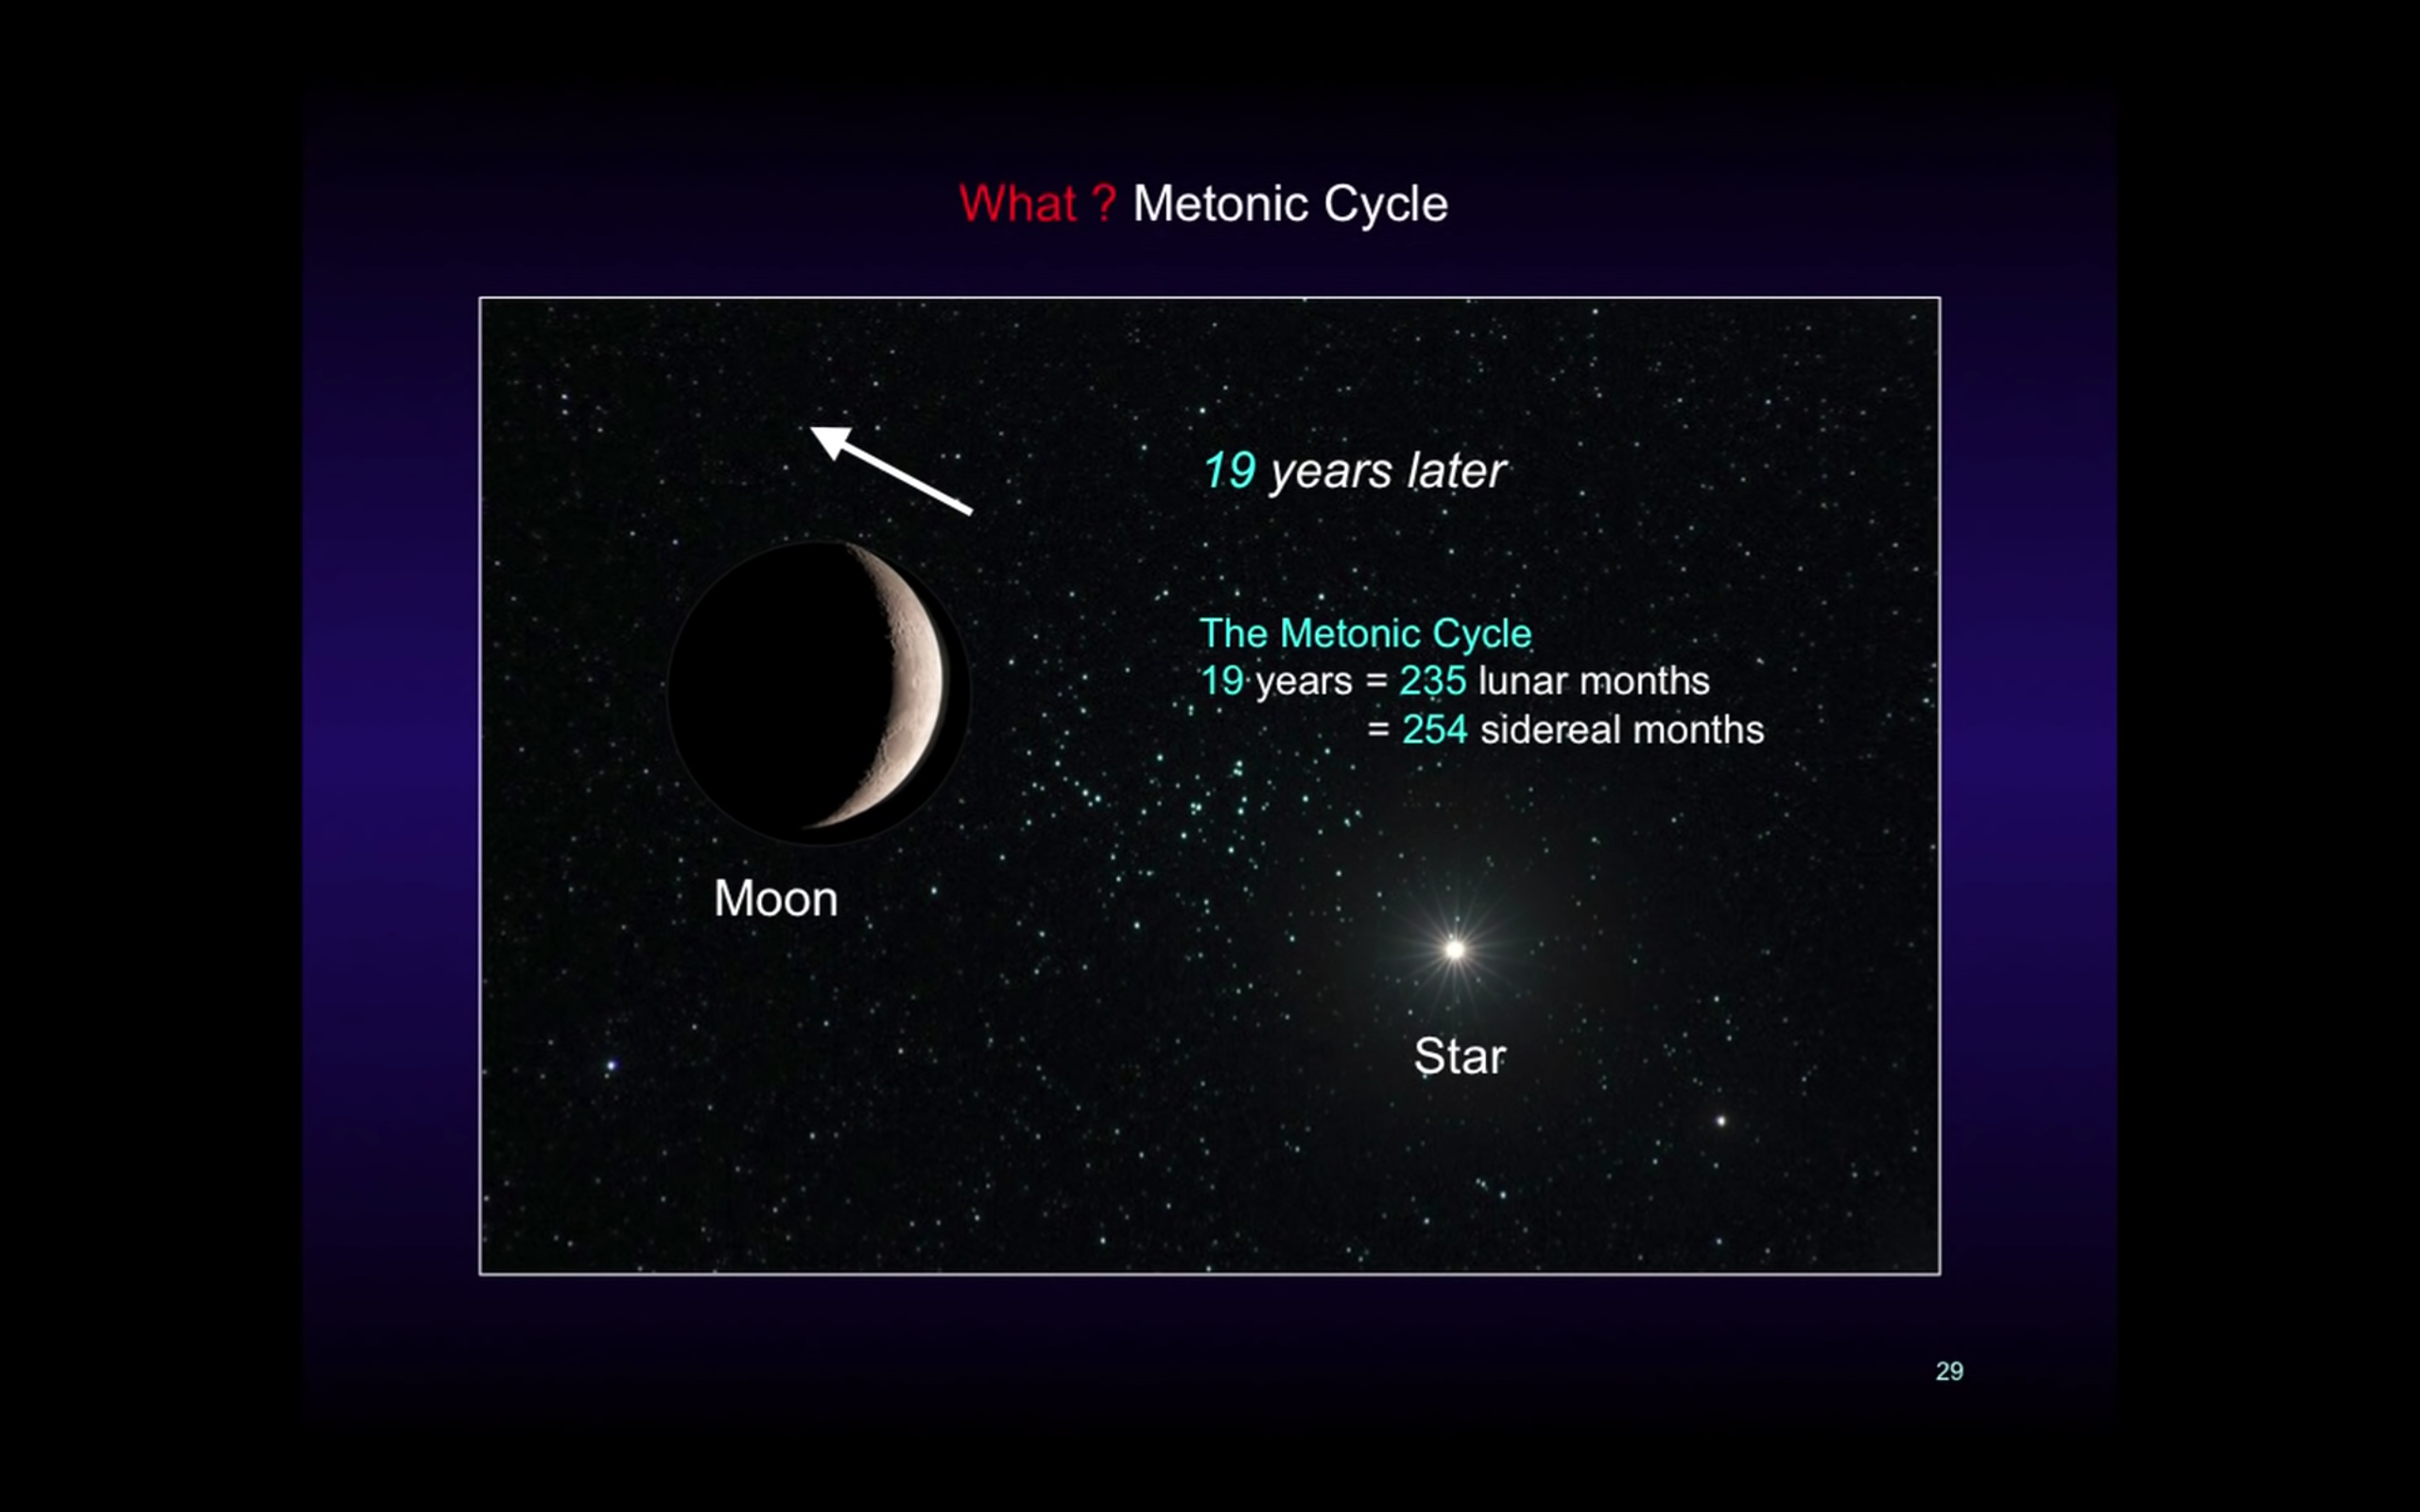
\includegraphics[scale=0.25,cfbox=red] {images/metonic.png}}
  \caption{The Metonic Cycle \cite{youtube:freeth2021}}
  \label{fig:metonic_cycle}
\end{figure}

\bigskip
\bigskip
\noindent
All very interesting but the Metonic Cycle seems to be a coincidence. The periods of the Moon's orbit around the Earth and the Earth's 
orbit around the Sun are believed to be independent, and not to have any known physical resonance. An example of a non-coincidental 
cycle is the orbit of Mercury, with its 3:2 spin-orbit resonance.

\section{Price's Metonic Gearing Scheme}
The purpose of the Metonic Cycle gearing scheme (which Price discovered) is to turn the (theorized) Moon output pointer such that it follows the Metonic Cycle.
Price's Metonic gearing scheme, described in his classic work "Gears from the Greeks. The Antikythera Mechanism: A Calendar Computer from ca. 80 B. C. T" \cite{gears_from_the_greeks}, 
is shown in Figure \ref{fig:general_gearing_plan}. 

\bigskip
\begin{figure}[H]
\center{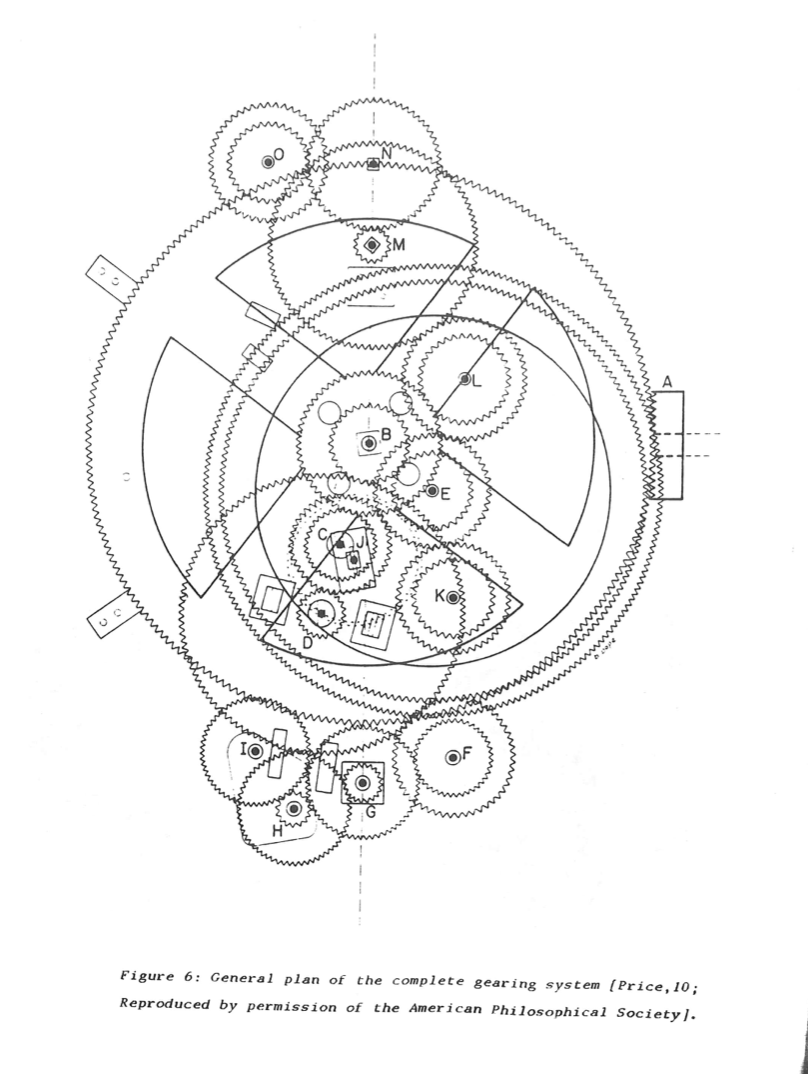
\includegraphics[scale=0.65,frame] {images/general_gearing_plan.png}}
\caption{Price's General Gearing Plan \cite{gears_from_the_greeks}}
\label{fig:general_gearing_plan}
\end{figure}

\bigskip
\noindent
For calculating gear ratios,  Price's sectional gearing diagram Figure \ref{fig:sectional_gearing} is more useful. As we can see from Figure \ref{fig:sectional_gearing}, the gears of interest
are B2, C1, C2, D1, D2, and E2, with the following tooth counts\footnote{The tooth counts were controversial in the 1950s when Price did much of his work.}:

\newpage

\begin{figure}[H]
  \center{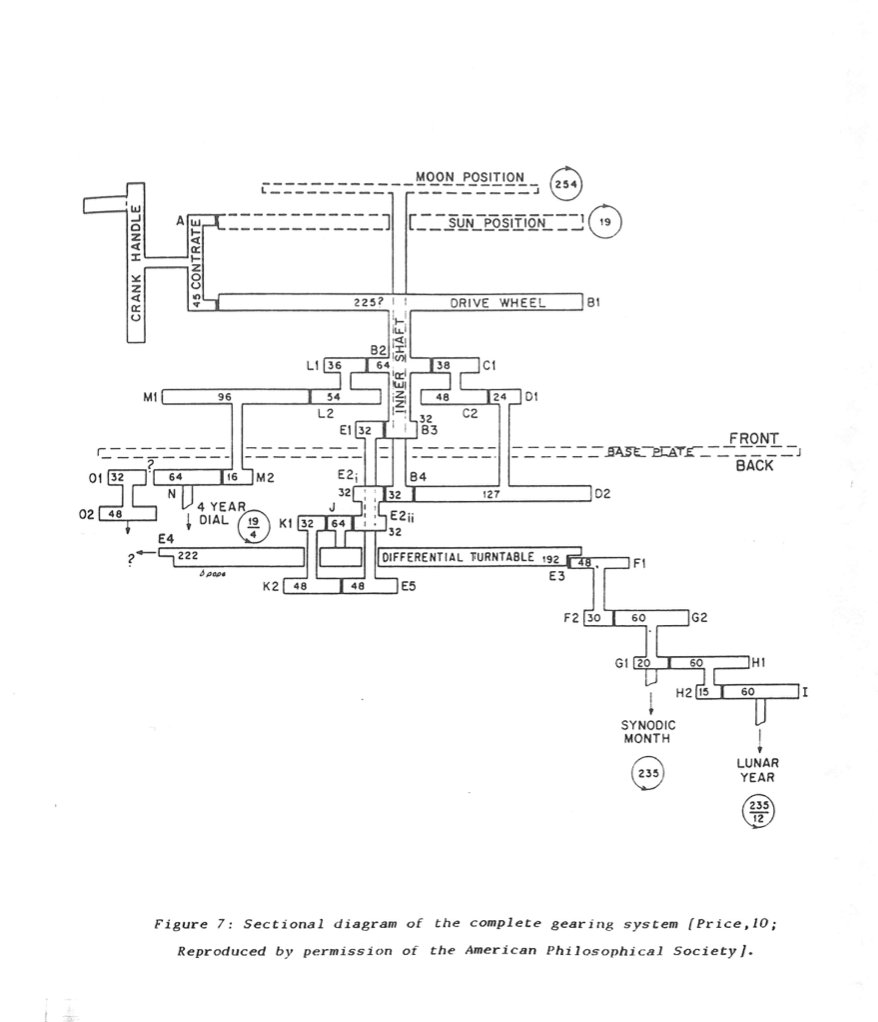
\includegraphics[scale=0.65,frame] {images/sectional_diagram.png}}
  \caption{Price's Sectional Gearing Diagram \cite{gears_from_the_greeks}}
  \label{fig:sectional_gearing}
\end{figure}
\bigskip
\bigskip
\bigskip
\begin{minipage}[c]{0.45\textwidth}
  \begin{itemize}
    \item B2: 64 teeth
    \item C1: 38 teeth
    \item C2: 48 teeth
    \item D1: 24 teeth
    \item D2: 127 teeth
    \item E2: 32 teeth
  \end{itemize}
\end{minipage}
\hfill
\begin{minipage}[c]{0.5\textwidth}
  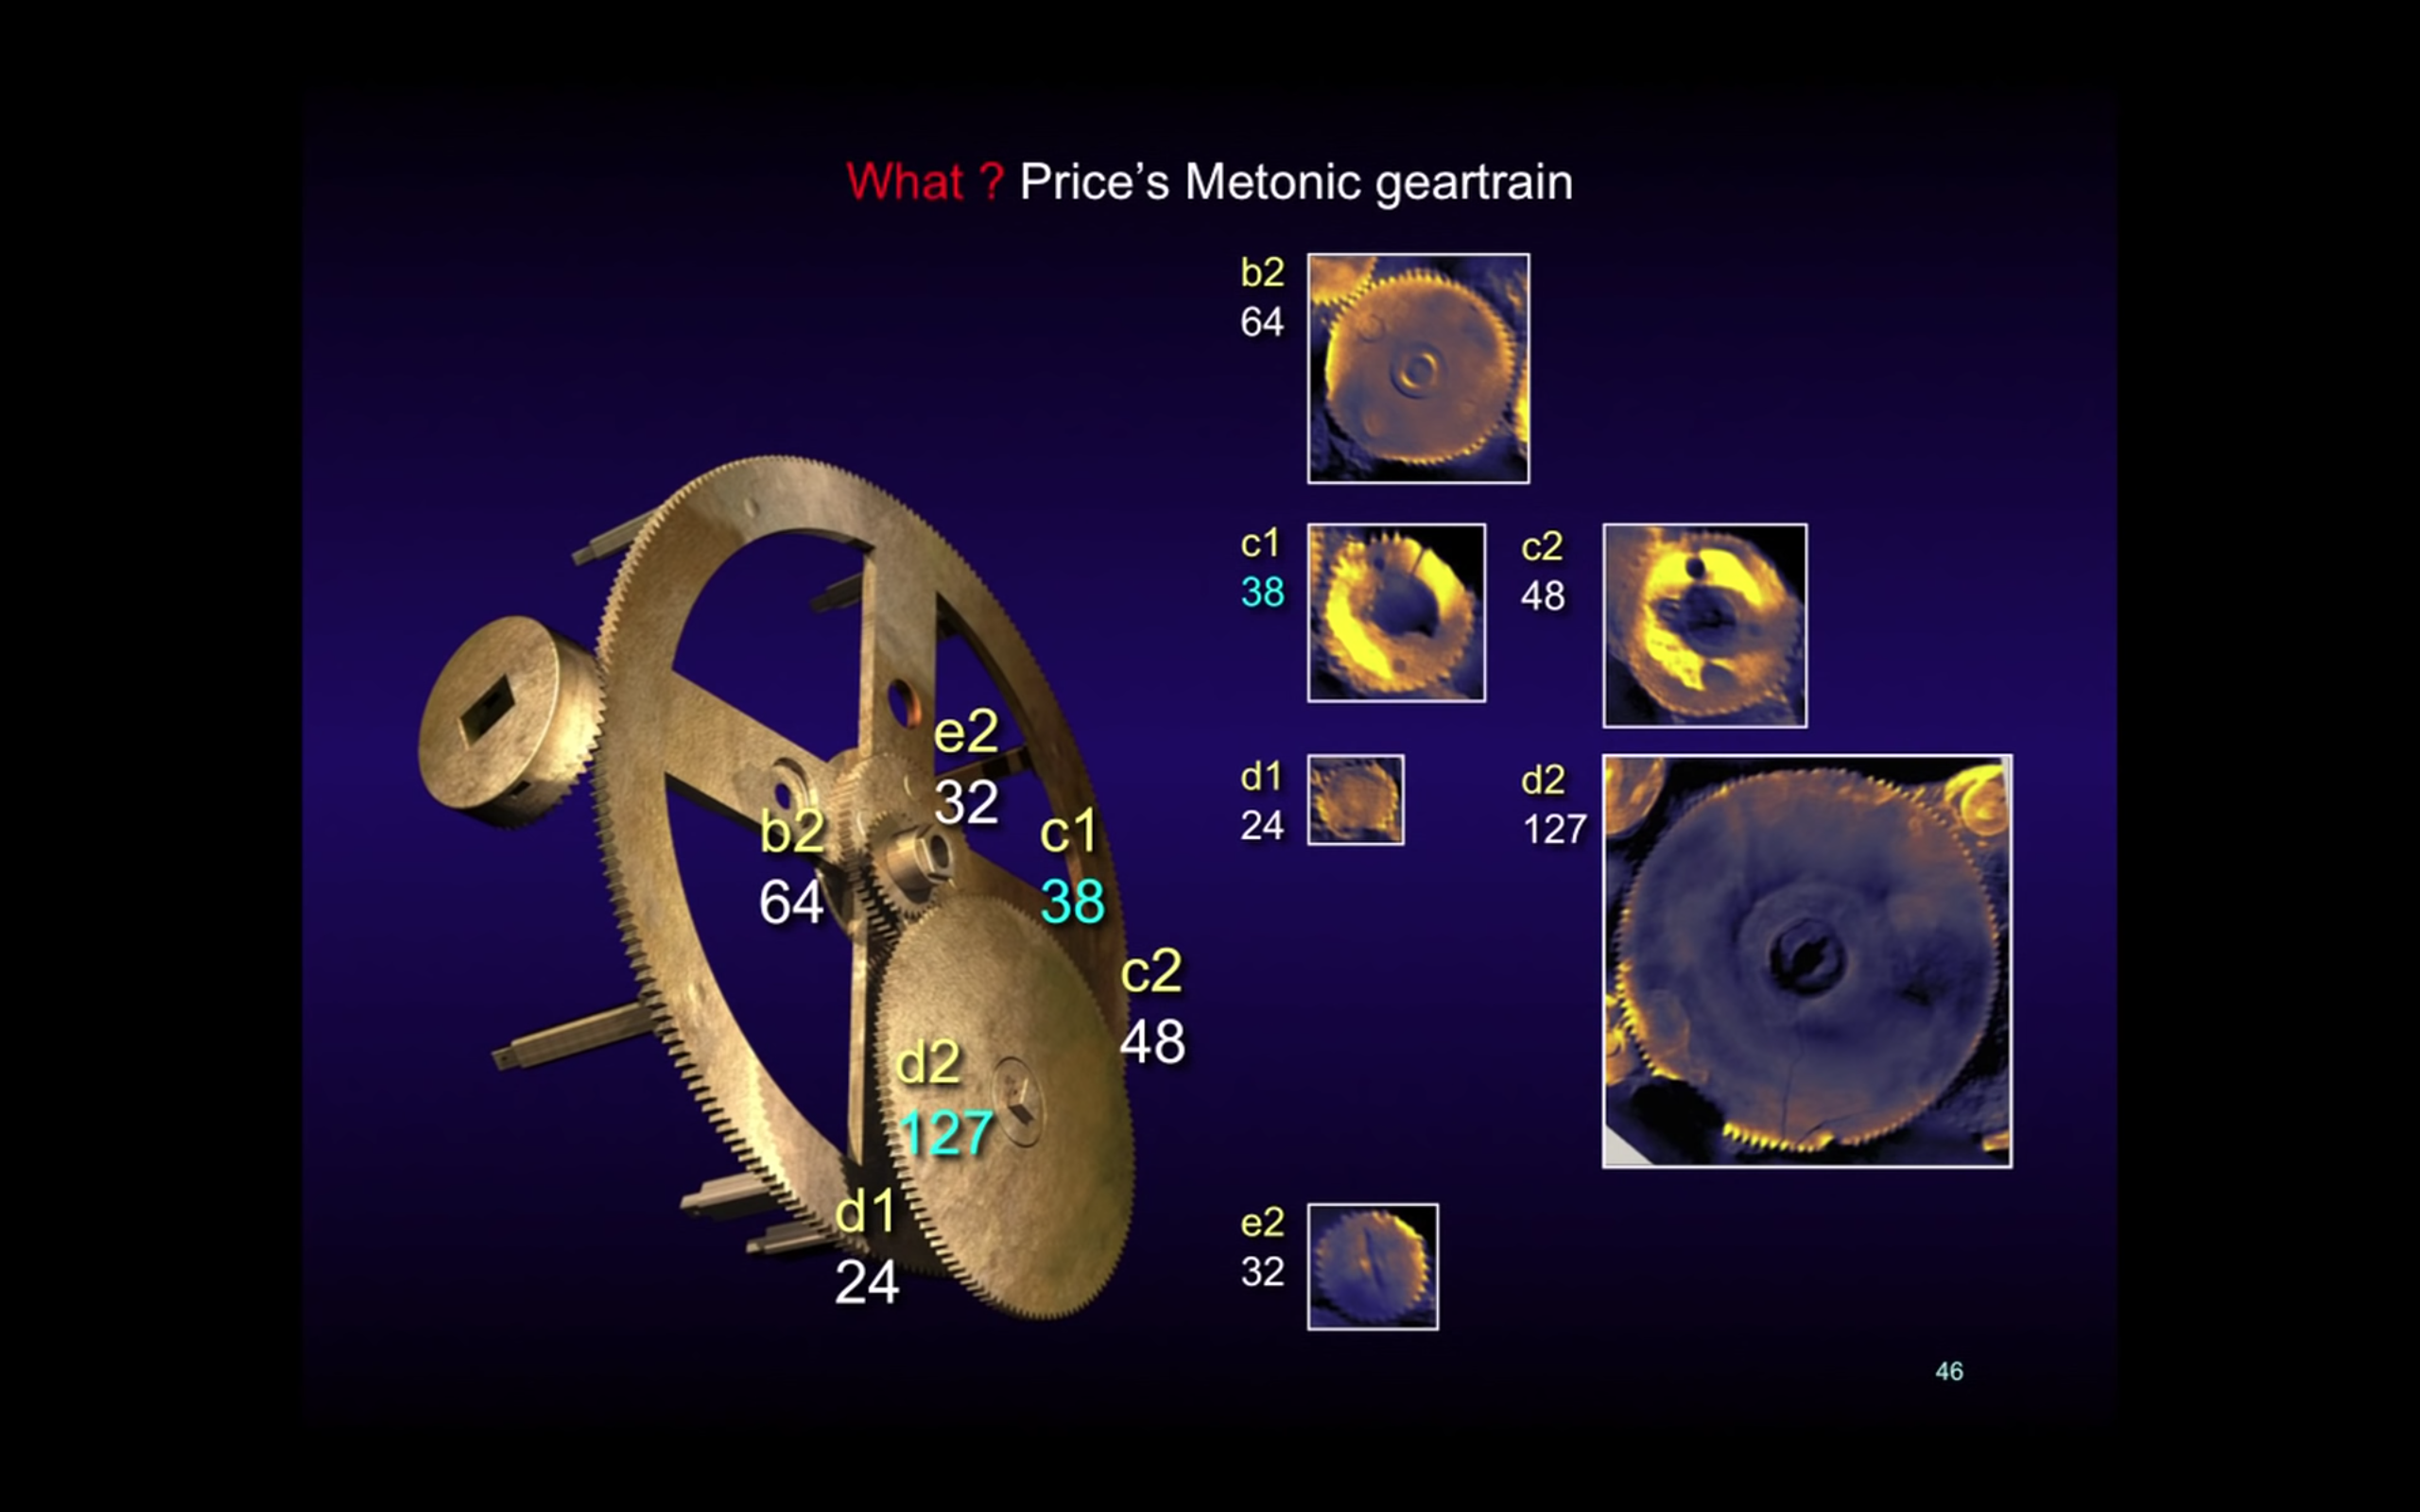
\includegraphics[width=\textwidth,cfbox=red]{images/price_metonic_gear_train.png}
  \captionof{figure}{The Metonic Gear Train \cite{youtube:freeth2021}}
\end{minipage}

\newpage

\bigskip
\noindent
We know that in simple gear trains we can calculate the Gear Ratio (GR) as 

\bigskip
\begin{center}
{\Large $\text{GR} = \frac{\text{Number of Teeth on the Driven Gear}}{\text{Number of Teeth on the Driver Gear}}$}
\end{center}

\bigskip
\noindent
and we know that the driven gear rotates in the opposite direction of the driver gear. 


\bigskip
\noindent
With this information we can start to calculate what Price's Metonic gear train does. 

\bigskip
\noindent
Specifically:

\begin{equation*}
\begin{array}{lllll}
\frac{\text{B2}}{\text{C1}} &= - \frac{64}{38} = - \frac{32}{19} & \quad \mathrel{\#} \text{driver \& driven gears turn in opposite directions} \\ \\
\frac{\text{B2}}{\text{C1}} \times \frac{\text{C2}}{\text{D1}} &= - \frac{64}{38} \times - \frac{48}{24} = - \frac{32}{19} \times - \frac{2}{1} = \frac{64}{19} 
& \quad \mathrel{\#} \frac{\text{C2}}{\text{D1}} \text{ multiplies $\frac{\text{B2}}{\text{C1}}$ by $2$}                       \\ \\
\frac{\text{B2}}{\text{C1}} \times \frac{\text{C2}}{\text{D1}} \times - \frac{\text{D2}}{\text{E1}} &= - \frac{64}{38} \times - \frac{48}{24} \times - \frac{127}{32} 
=  -\frac{254}{19} & \quad \mathrel{\#} \frac{254}{19} \approx 13.36842
\end{array}
\end{equation*}


\bigskip
\begin{figure}[H]
\center{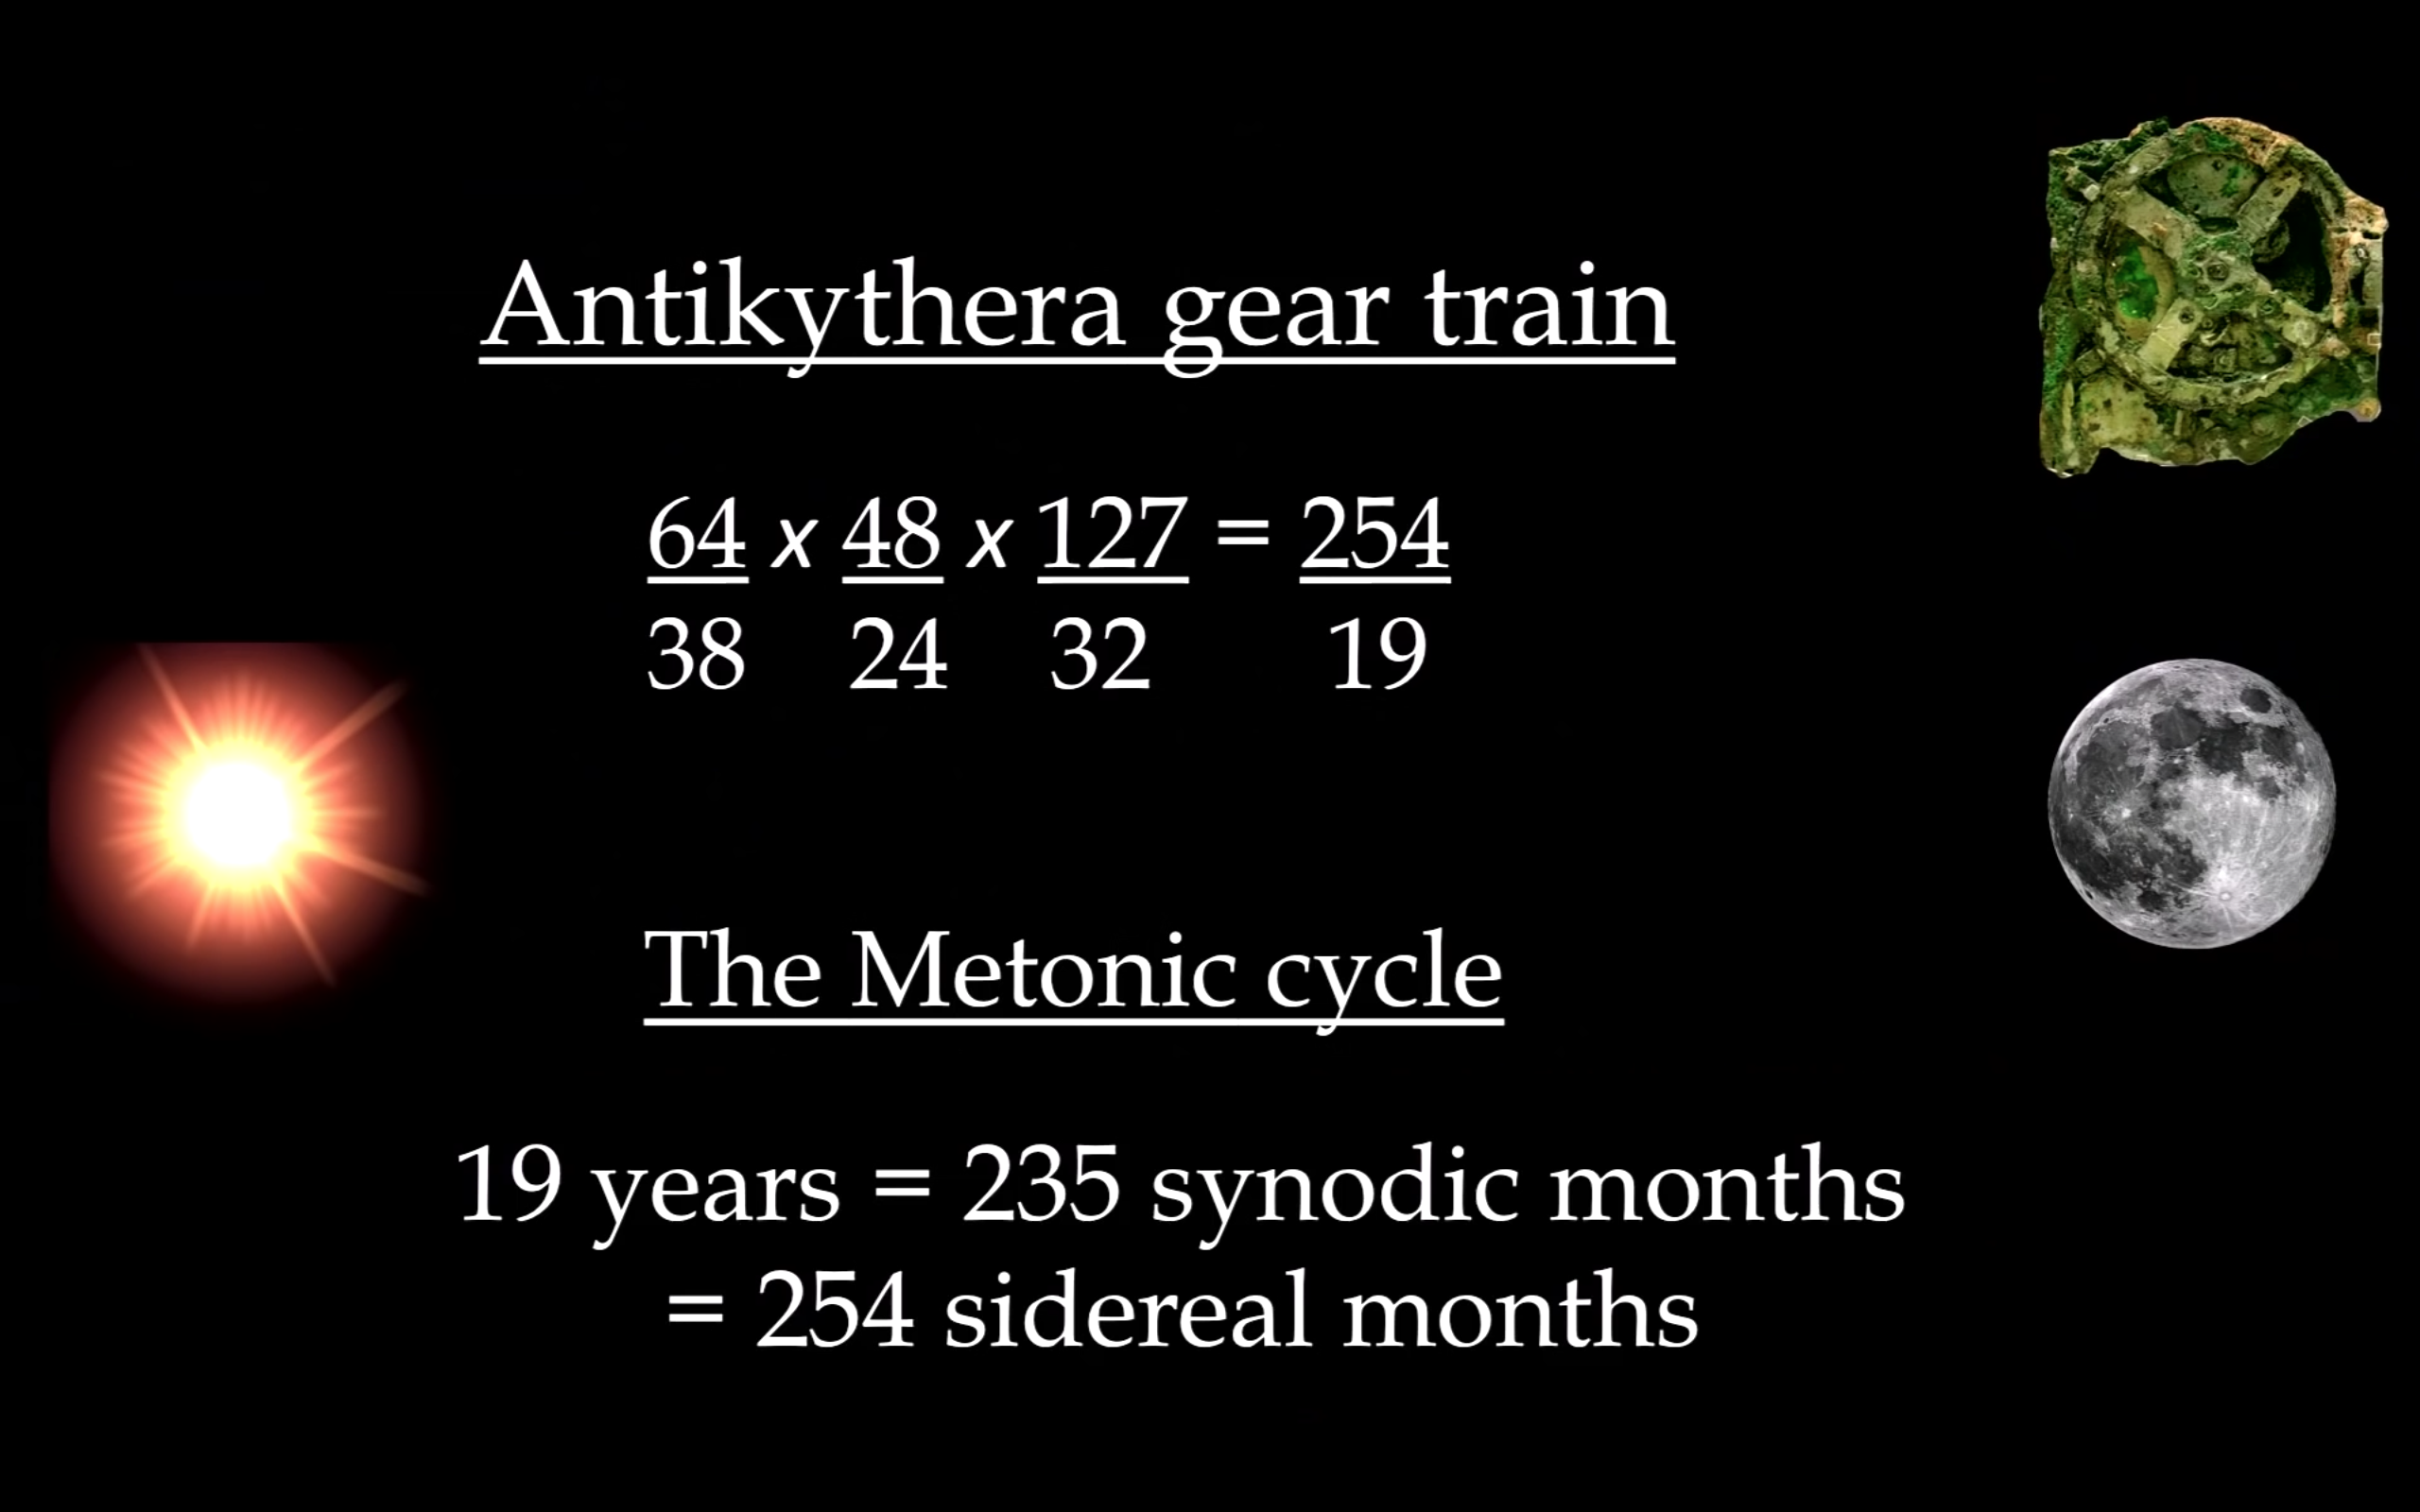
\includegraphics[scale=0.20,cfbox=red] {images/price_gear_train.png}}
\caption{Metonic Gear Train Ratios and the Metonic Cycle}
\label{fig:metonic_gear_ratios}
\end{figure}

\bigskip
\section{Acknowledgements}

\newpage
\bibliographystyle{plain}
\bibliography{/Users/dmm/papers/bib/astronomy}
\end{document} 
